% ------------------------------------------------------------------------------------
\newpage
{\color{lightgray} \hrule}
\begin{enumerate} \setcounter{enumi}{1}
	\item Considere los tiempos de falla $t_1, \dots, t_n$ con distribución $Weibull(\alpha, \lambda)$:
	\begin{equation} \label{eq:7}
		f(t_i | \alpha, \lambda) = \alpha \lambda t_{i} ^{\alpha-1} e^{-t_{i}^{\alpha}\lambda}
	\end{equation}
	Se asumen como a priori $\alpha \sim exp(c)$ y $\lambda|\alpha \sim Gama(\alpha, b)$, por lo tanto, $f(\alpha, \lambda) = f(\lambda|\alpha) f(\alpha)$. Así, para la distribución posterior se tiene:
	\begin{equation} \label{eq:8}
		f(\alpha,\lambda|\bar{t}) \propto f(\bar{t}|\alpha, \lambda) f(\alpha, \lambda)
	\end{equation}
	A partir del algoritmo MH usando Kerneles híbridos simule valores de la distribución posterior $f(\alpha, \lambda | \bar{t})$, considerando las siguientes propuestas:
	\begin{itemize}
		\item Propuesta 1:
		\begin{equation} \label{eq:9}
			\lambda_p | \alpha, \bar{t} \sim Gama \left( \alpha+n, b+\sum_{i=1}^{n} t_i^{\alpha} \right) \text{ y dejando $\alpha$ fijo}.
		\end{equation}
		\item Propuesta 2:
		\begin{equation} \label{eq:10}
			\alpha_p | \lambda, \bar{t} \sim Gama \left( n+1, -\log{b} - \log{r_1} + c \right) \text{ con } r_1 = \prod_{i=1}^{n} t_i \text{ y dejando $\lambda$ fijo}.
		\end{equation}
		\item Propuesta 3:
		\begin{equation} \label{eq:11}
			\alpha_p \sim exp(c) \textit{ y } \lambda_p|\alpha_p\sim Gama(\alpha_p,b)
		\end{equation}
		\item Propuesta 4 (RWMH):
		\begin{equation} \label{eq:12}
			\alpha_p = \alpha + \epsilon \text{, con } \epsilon\sim\mathcal{N}(0,\sigma) \text{ y dejando $\lambda$ fijo}.
		\end{equation}
		Simular datos usando $\alpha=\lambda=1$ con $n= 30$. Para la a priori usar $c= 1$ y $b= 1$.
	\end{itemize}
\end{enumerate}

\textcolor{BrickRed}{\it Respuesta:}

En el archivo \textcolor{mediumblue}{ejercicio2\_tarea8.py}, se comienza implementando la función \textit{plot\_chains()}, la cual recibe una cadena de Markov simulada y grafica el histograma de cada variable, además, traza los valores reales de $\alpha$ y $\beta$, que en ejercicio se piden ambos igual a $1$. Gracias a lo general que es la función \textit{METROPOLIS\_HASTINGS\_HYBRID\_KERNELS()} descrita en el ejercicio anterior, se vuelve a usar sin hacer ninguna modificación.

A continuación, se define la función \textit{posterior()} la cual implementa la expresión \eqref{eq:8} y las propuestas:
\begin{itemize}
	\item \textit{prop1\_gen()}  y \textit{prop1\_pdf()}
	\item \textit{prop2\_gen()} y \textit{prop2\_pdf()}
	\item \textit{prop3\_gen()}  y \textit{prop3\_pdf()}
	\item \textit{prop4\_gen()} y \textit{prop4\_pdf()}
\end{itemize}
las cuales implementan las propuestas \eqref{eq:9}, \eqref{eq:10}, \eqref{eq:11} y \eqref{eq:12} así como su densidad de probabilidad respectiva. En estas funciones es importante notar que se respeta cuando se deja fija alguna de las variables ($\alpha$ en la propuesta $1$ y  $\lambda$ en la propuesta $2$ y $4$).

Finalmente, se ejecuta el código principal, en el cual se definen los parámetros dados por el ejercicio, como $\alpha=\lambda=b=c=1$ y $n= 30$. Además, para la propuesta $4$, se usa $\sigma=0.1$ gracias a que se obtuvieron buenos resultados con este valor. El punto $x_0$ inicial se tomó aleatorio en $[0,1]$ por simplicidad y se usaron $10,000$ iteraciones del algoritmo. Además, se le dio igual probabilidad de elección a cada una de las propuestas: $\frac{1}{4}$. Así, se generaron las observaciones $t$ de la distribución Weibull para luego generar las listas de funciones generadoras y sus respectivas densidades para aplicar el algoritmo Metropolis Hastings con Kérneles Híbridos generando los resultados mostrados a continuación:

\begin{figure}[h!]
	\centering
	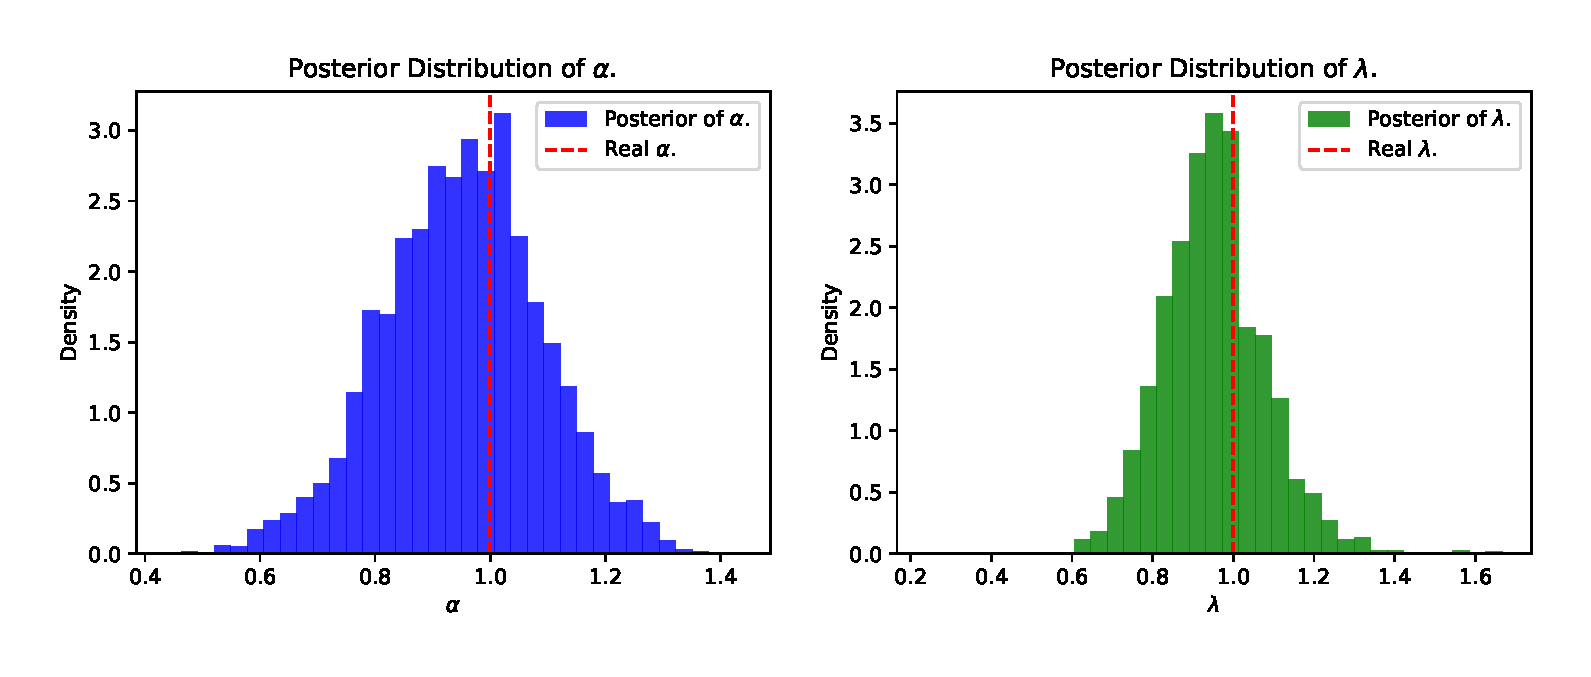
\includegraphics[width=\textwidth]{IMAGENES/exercise2.pdf}
\end{figure}

Podemos notar que las estimaciones para $\alpha$ y $\lambda$ fueron bastante buenas, ya que las distribuciones tienen sus medias muy cerca a los valores reales $\alpha=\lambda=1$. Este resultado se repitió en varias ocasiones para distintos valores de los parámetros y número de iteraciones, en particular, parecía invariante a la elección de la desviación estándar $\sigma$ de la propuesta $4$.